% !TEX program = xelatex
% 中心科学实验 IV 研究型实验报告模板
% 化学国家级实验教学示范中心（厦门大学）

\documentclass[a4paper]{article}

% ===== 字体 =====
\usepackage{fontspec}
\usepackage{xeCJK}
\setCJKmainfont[BoldFont=SimHei]{SimSun}      % \textbf 中文 → 黑体
\setCJKsansfont[BoldFont=SimHei]{SimHei}
\setCJKmonofont{FangSong}
\newCJKfontfamily\heiti[BoldFont=SimHei]{SimHei}
\newCJKfontfamily\kaishu{KaiTi}
\newCJKfontfamily\fangsong{FangSong}
\newCJKfontfamily\xingkai{STXingkai}
% 开启假粗体后备（对没有显式 BoldFont 的字体合成加粗）
\xeCJKsetup{AutoFakeBold=true}
\setmainfont{Times New Roman}

% ===== 字号定义 =====
\newcommand{\zihaoSan}{\fontsize{16pt}{24pt}\selectfont}
\newcommand{\zihaoSi}{\fontsize{14pt}{21pt}\selectfont}
\newcommand{\zihaoWu}{\fontsize{10.5pt}{16pt}\selectfont}
\newcommand{\zihaoXiaoWu}{\fontsize{9pt}{13.5pt}\selectfont}
\newcommand{\zihaoLiu}{\fontsize{7.5pt}{11pt}\selectfont}

% ===== 正文行距 =====
% 10.5pt字体，行距16pt，linespread=16/(10.5*1.2)=1.2698
\usepackage{setspace}

% ===== 页面 =====
\usepackage[a4paper,
  top=4.6cm, bottom=3.0cm,
  left=2.5cm, right=2.0cm,
  headheight=3.8cm,
  headsep=0.8cm,
  footskip=1.8cm]{geometry}

% ===== 页眉页脚 =====
\usepackage{fancyhdr}
\usepackage{graphicx}

\newcommand{\infobar}{%
  \zihaoWu
  \setlength{\tabcolsep}{0pt}%
  \vspace{0.5em}
  \begin{tabular}{@{}p{0.315\textwidth}p{0.315\textwidth}p{0.315\textwidth}@{}}
    系（Dept.）\underline{\hspace{2.2cm}} &
    专业（Major）\underline{\hspace{1.3cm}} &
    学号（ID）\underline{\hspace{1.3cm}} \\[7pt]
    姓名（Name）\underline{\hspace{1.6cm}} &
    日期（Date）\underline{\hspace{1.5cm}} &
    实验台号（No.）\underline{\hspace{0.8cm}}
  \end{tabular}%
  \vspace{1em}
}

\newcommand{\myhead}{%
  \begin{minipage}[c]{2cm}%
    
\includegraphics[height=2cm]{images/img-000.png}%
  \end{minipage}%
  \vspace{-0.5em}%
  \begin{minipage}[c]{\dimexpr\textwidth-1.8cm\relax}%
    \centering
    {\hspace{-1.5em}\zihaoSan\heiti 中心科学实验 IV\hspace{2em}{\xingkai 实\kern0.2em 验\kern0.2em 报\kern0.2em 告}}\\[3pt]
    {\hspace{-1.5em}\fontsize{11pt}{14pt}\selectfont\textbf{Experimental Report of Central Science}}\\[6pt]
    \infobar
  \end{minipage}%
}

\pagestyle{fancy}
\fancyhf{}
\renewcommand{\headrulewidth}{0.4pt}
\renewcommand{\footrulewidth}{0.4pt}
\fancyhead[L]{\myhead}
\fancyfoot[C]{
  \vspace{-0.5em}
  \zihaoWu \bfseries 化学国家级实验教学示范中心（厦门大学）\\[1pt]
  {\textbf{\fontsize{9pt}{13pt}\selectfont
    National Demonstration Center for Experimental Chemistry Education (Xiamen University)}}
}

\fancypagestyle{plain}{%
  \fancyhf{}
  \renewcommand{\headrulewidth}{0.4pt}
  \renewcommand{\footrulewidth}{0.4pt}
  \fancyhead[L]{\myhead}
  \fancyfoot[C]{
    \vspace{-0.5em}
    \zihaoWu \bfseries 化学国家级实验教学示范中心（厦门大学）\\[1pt]
    {\textbf{\fontsize{9pt}{13pt}\selectfont
      National Demonstration Center for Experimental Chemistry Education (Xiamen University)}}
  }
}

% ===== 标题样式 =====
\usepackage{titlesec}
\titleformat{\section}{\zihaoSi\heiti}{\thesection}{1em}{}
\titlespacing{\section}{0pt}{12pt}{6pt}
\titleformat{\subsection}{\zihaoWu\heiti\bfseries}{\thesubsection}{1em}{}
\titlespacing{\subsection}{0pt}{0pt}{0pt}

% ===== 表格图片 =====
\usepackage{booktabs}
\usepackage{multirow}
\usepackage{caption}
\captionsetup[table]{labelsep=space,font={small},position=above,skip=4pt,justification=centering}
\captionsetup[figure]{labelsep=space,font={small},position=below,skip=4pt,justification=centering}
\renewcommand{\figurename}{图}
\renewcommand{\tablename}{表}
\renewcommand{\refname}{参考文献}

% ===== 参考文献 =====
\usepackage[super,sort&compress]{natbib}
\bibliographystyle{unsrt}

% ===== 其他 =====
\usepackage[colorlinks=true,linkcolor=black,urlcolor=blue,citecolor=black]{hyperref}
\usepackage{indentfirst}
\setlength{\parindent}{2em}
\setlength{\parskip}{0pt}
\usepackage{enumitem}
\setlist{nosep}

% ======================================================
% 评语与签字栏（整体不分页，置于最末）
\usepackage{needspace}

% ======================================================

\usepackage{hyperref}

\begin{document}

\setstretch{1.05}
\zihaoWu

\begin{center}
  {\zihaoSan\heiti 纳米颗粒光学显微成像}
\end{center}

\vspace{6pt}

\section{引言}
\vspace{-0.5em}

金、银等贵金属纳米颗粒的光学响应与尺寸、形貌及周围介质密切相关。入射光可驱动纳米颗粒表面自由电子发生集体振荡，形成局域表面等离子体共振（localized surface plasmon resonance, LSPR）。LSPR 峰位和散射颜色会随颗粒粒径、组成及各向异性形貌改变而发生变化，因此单颗粒光学成像可作为纳米材料快速识别和生物体系原位观察的重要手段\cite{eustis2006,murphy2005}。

暗场显微镜利用斜入射照明阻挡直射光，仅收集样品散射、反射或衍射进入物镜的光。由于背景近似为黑色，暗场成像对纳米颗粒、细胞轮廓及活体体系中微小散射体具有较高对比度，能够在不引入荧光标记的情况下观察颗粒的存在和运动。对于细胞膜表面或细胞内的纳米颗粒，其运动轨迹包含扩散状态、受限程度和可能的内吞转运信息。单颗粒追踪结合均方位移（mean square displacement, MSD）分析，可区分近似自由扩散、受限扩散和异常扩散等模式\cite{kusumi1993,kowalek2019}。

本实验利用暗场显微成像观察不同形貌金属纳米颗粒的散射颜色和形状特征，并进一步追踪纳米颗粒在细胞膜相关区域的运动轨迹，计算表观扩散参数和异常扩散指数，从而讨论纳米颗粒光学性质与结构、细胞界面相互作用之间的联系。


\section{实验部分}
\vspace{-0.5em}

\subsection{仪器与试剂}

实验试剂与材料包括纳米金分散液、纳米银分散液、PBS 缓冲液、F-12K 培养基、细胞样品、超纯水、载玻片、盖玻片、剪刀、镜油、擦镜纸、双面胶和指甲油等。其中 PBS 和 F-12K 培养基分别用于颗粒稀释和细胞样品腔室中的液相环境维持；镜油用于暗场聚光镜、载玻片和油镜之间的光学耦合；指甲油用于封片，减少样品蒸发和液体流动。

主要仪器包括 Nikon-NIE、Nikon-80i 显微镜系统、白光光源、暗场聚光镜、60 倍物镜、CMOS 相机、微型孵化器、移液枪以及 ImageJ 数据处理软件。暗场显微镜的关键部件为暗场聚光镜，其作用是使照明光以空心锥形光束斜入射到样品上，阻挡中心直射光，使未被样品散射的光不进入物镜；当样品中的纳米颗粒、细胞边缘或细胞内结构改变光路方向时，散射光进入物镜形成明亮图像。

\subsection{实验方法}

\subsubsection{暗场显微镜的调节与使用}

实验开始前打开显微镜电源与白光光源，依次安装暗场聚光镜和 60 倍物镜，并用擦镜纸清洁镜头及玻片表面。将暗场聚光镜上调至接近载物台下缘后，在聚光镜中央滴加镜油。将玻片样品缓慢推入压片夹，使待观察区域正对通光孔；随后在盖玻片上方观察区域滴加少量镜油，使物镜与盖玻片之间形成连续油层。调焦时先观察物镜与玻片间距，避免镜头压碎玻片，再通过粗准焦螺旋接近焦面，最后用细准焦螺旋获得清晰暗场图像。观察过程中若背景不够黑或亮斑不清晰，需要重新调整聚光镜高度、油层接触和照明中心。

\subsubsection{不同纳米颗粒的暗场成像}

待测纳米颗粒分散液在使用前进行超声分散，以减少颗粒聚集。取 10~$\mu$L 颗粒分散液与 40~$\mu$L PBS 缓冲液混合，得到约 5 倍稀释的样品，并继续超声约 10~min。随后在洁净载玻片上滴加约 10~$\mu$L 稀释液，小心覆盖盖玻片，用滤纸吸去多余液体并用指甲油密封。待封片稳定后，在暗场显微镜下记录颗粒的散射颜色、形状、亮度和运动状态。四种未知颗粒可依据点状或棒状形貌以及绿色、蓝色、黄色、橙红色等散射颜色进行判别。

\subsubsection{细胞样品观察与颗粒轨迹采集}

细胞样品制备时，在洁净载玻片上平行粘贴两条双面胶，将贴有细胞的盖玻片倒扣在双面胶上，使载玻片与盖玻片之间形成薄层腔室。取 10~$\mu$L 纳米颗粒分散液与 40~$\mu$L F-12K 培养基混匀后注入腔室，并用指甲油密封四周，防止培养基外流和蒸发。样品置于微型孵化器上，在 37~℃条件下孵育约 30~min，使颗粒有足够时间与细胞膜接触、吸附或发生内吞。随后使用暗场显微镜观察细胞轮廓、细胞内散射结构以及颗粒在细胞膜内外的分布，选择与细胞背景区分较好的亮点进行视频采集。

\subsubsection{数据处理}

使用 ImageJ 对采集视频中的单颗粒亮点进行轨迹提取。为降低细胞器强散射和固定背景亮点的干扰，追踪时需尽量选择信噪比较高、与邻近亮点不重叠且轨迹连续的颗粒。实验坐标按 246.8~nm/像素换算为实际长度，帧间隔为 0.02~s。对轨迹计算不同时间间隔下的均方位移（MSD），并使用
\[
  MSD(t)=4Dt^{\alpha}
\]
进行幂律拟合。其中 $D$ 为二维表观扩散参数，$\alpha$ 为异常扩散指数；$\alpha\approx1$ 表示接近自由布朗扩散，$0.5<\alpha<1$ 通常对应弱受限亚扩散，$\alpha<0.5$ 则说明颗粒受到更强限制或轨迹中存在明显停滞与局域束缚。

\section{结果与讨论}
\vspace{-0.5em}

\subsection{不同纳米颗粒的暗场成像鉴别}

暗场图像中纳米颗粒在黑色背景上呈现明亮散射光点或短棒状散射体。球形颗粒主要表现为点状散射，而金纳米棒因具有各向异性结构，可观察到更明显的短棒或长棒特征；同时，纳米棒纵向 LSPR 对长径比更敏感，长径比较大的颗粒散射峰发生红移，因而呈现更偏橙红的颜色。

\begin{figure}[htbp]
  \centering
  \begin{minipage}{0.47\linewidth}
    \centering
    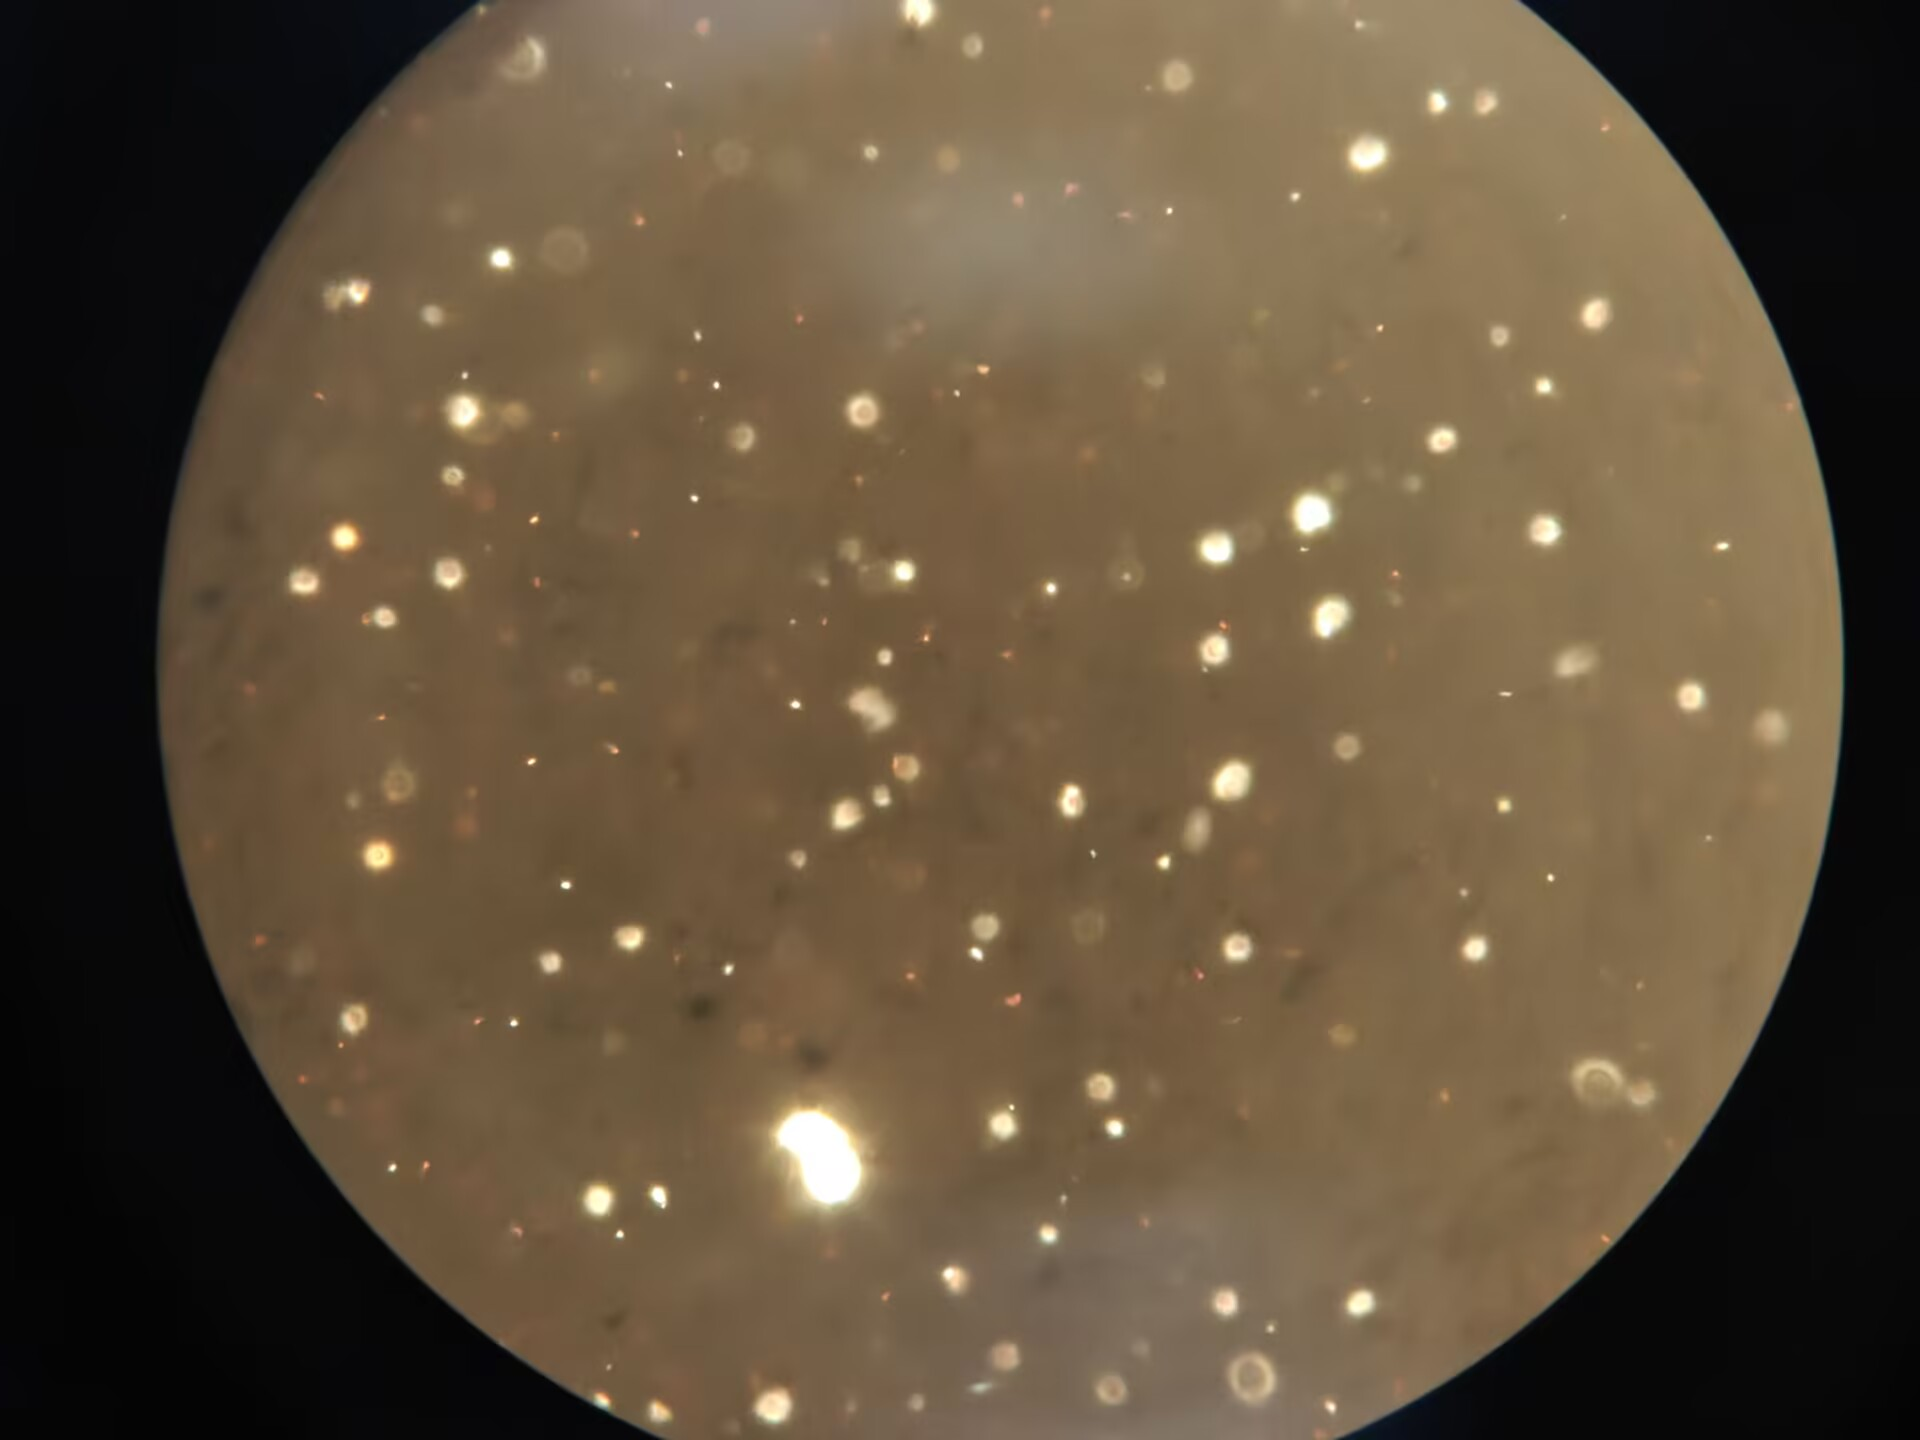
\includegraphics[width=\linewidth]{src/img/sample_particles_darkfield_3.jpg}
  \end{minipage}\hfill
  \begin{minipage}{0.47\linewidth}
    \centering
    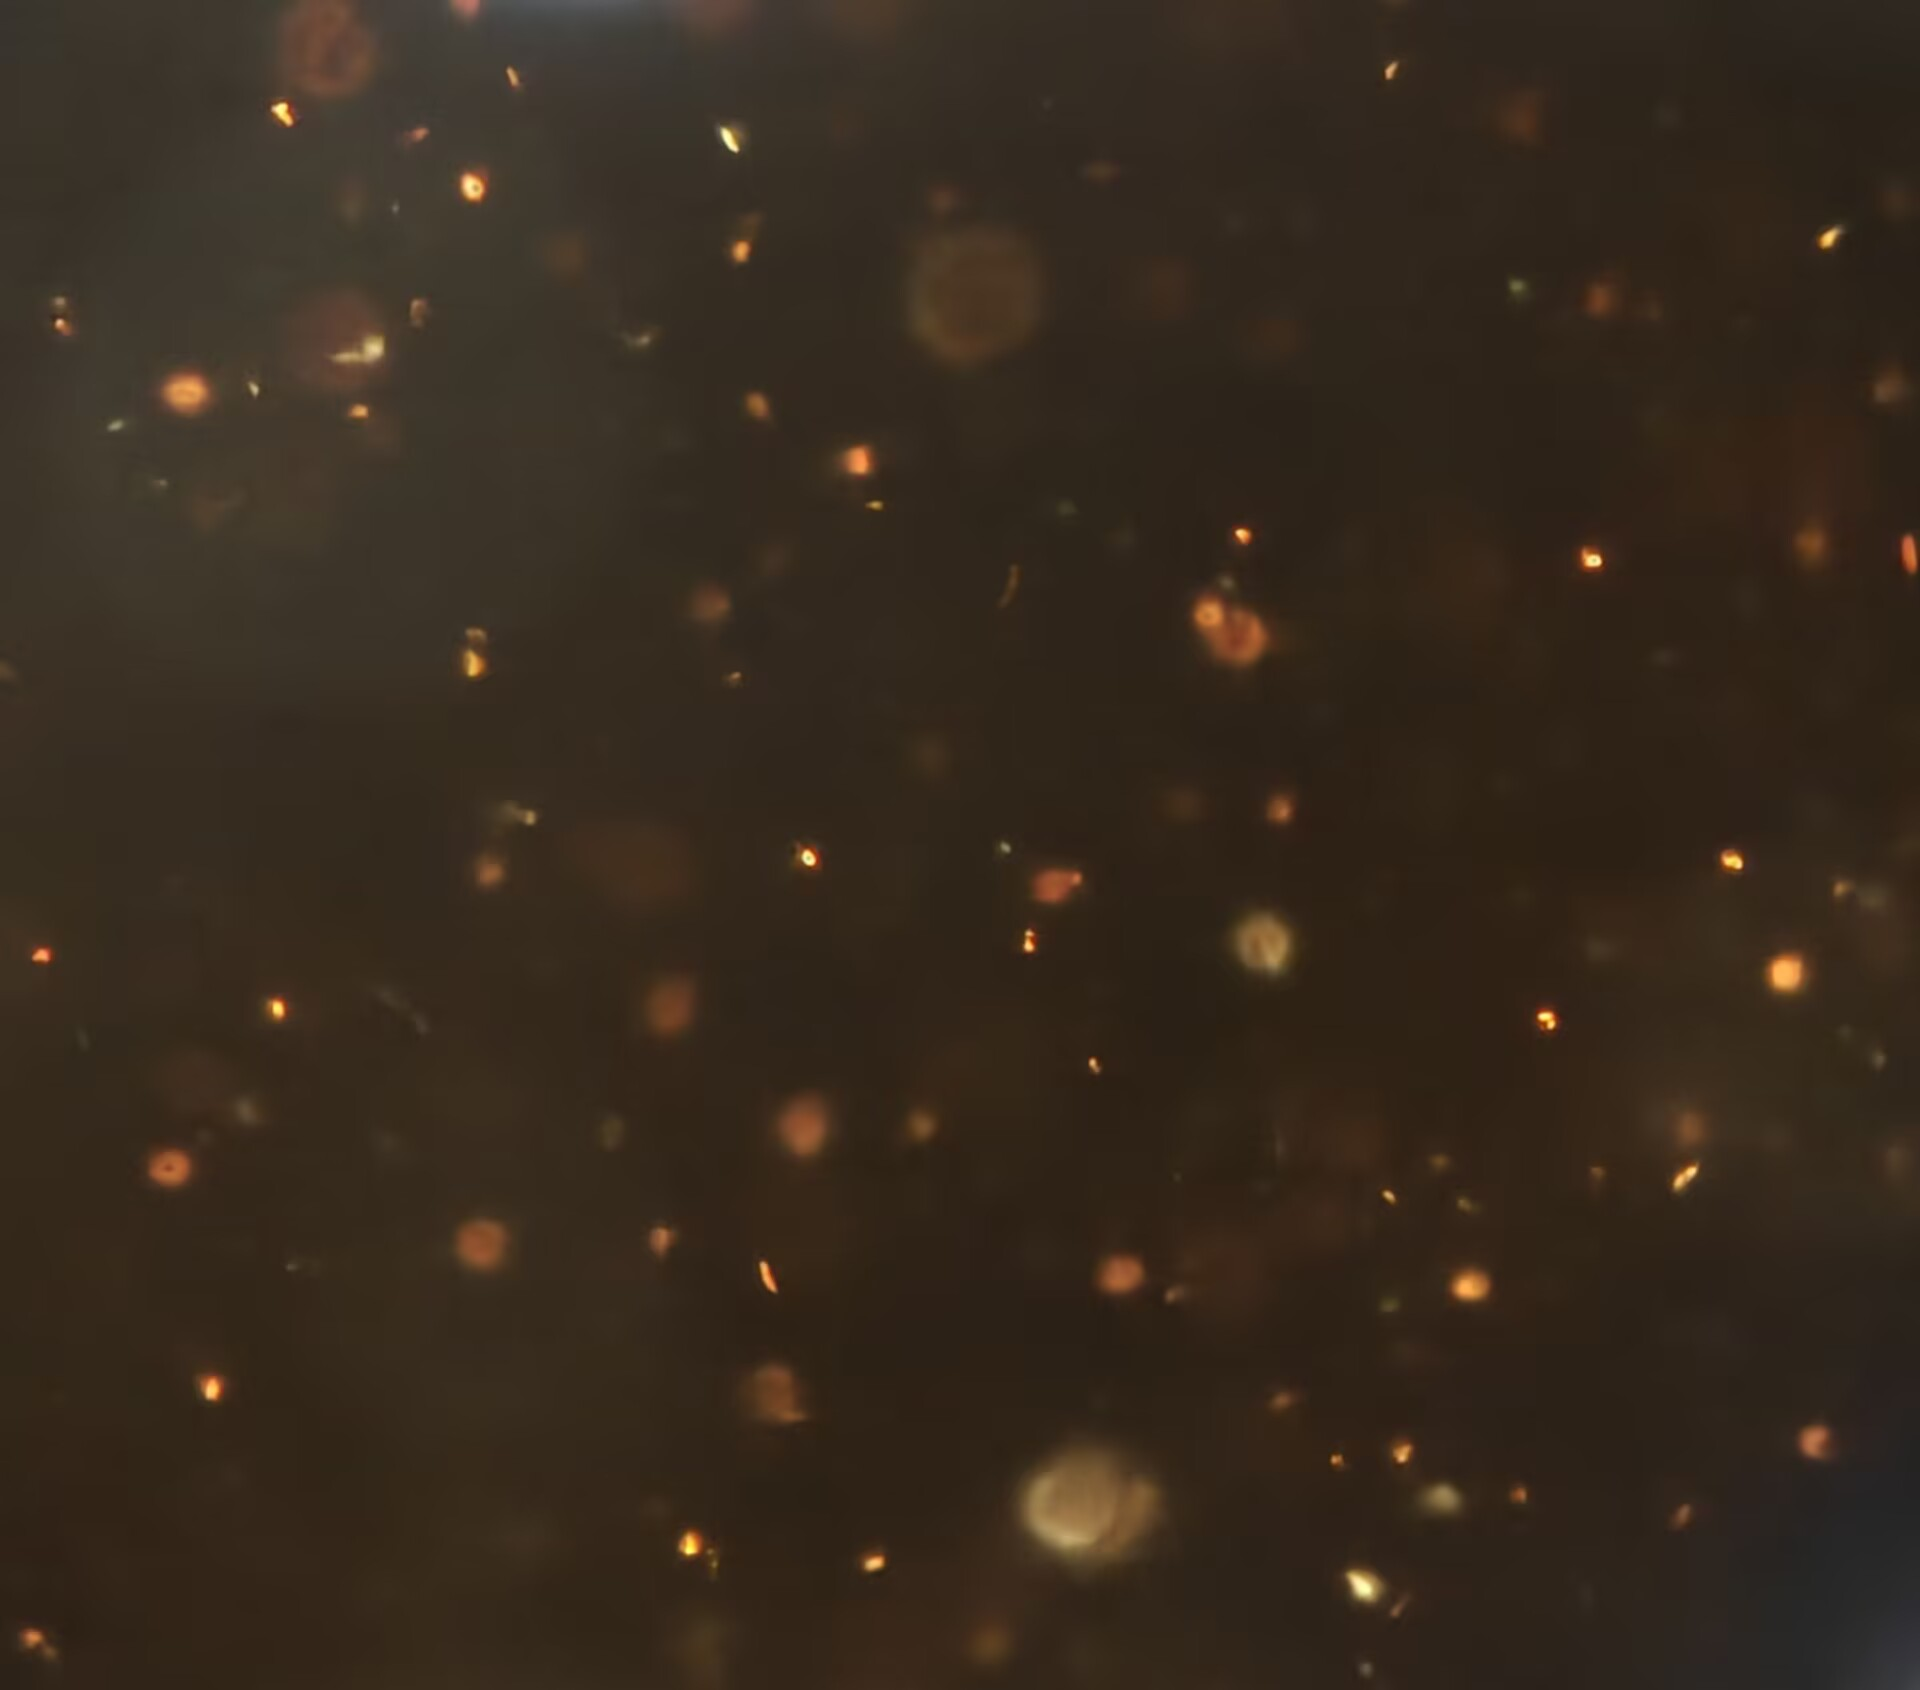
\includegraphics[width=\linewidth]{src/img/sample_particles_darkfield.jpg}
  \end{minipage}
  \caption{{\zihaoWu 不同纳米颗粒的暗场显微成像。点状和棒状散射体可分别对应球形纳米颗粒和纳米棒。}}
  \label{fig:cell}
\end{figure}

\begin{table}[htbp]
  \centering
  \caption{{\zihaoXiaoWu 暗场图像中不同纳米颗粒的形貌和散射颜色鉴别}}
  \label{tab:particle_id}
  {\zihaoLiu
    \begin{tabular}{cccc}
      \toprule
      观察特征  & 推断样品                 & 主要形貌 & 判据                 \\
      \midrule
      绿色点状  & 55~nm 金纳米颗粒          & 球形颗粒 & 点状散射，LSPR 位于绿光附近   \\
      蓝色点状  & 60~nm 金纳米颗粒          & 球形颗粒 & 点状散射，颜色较短波         \\
      黄色短棒  & 25$\times$60~nm 金纳米棒 & 短棒   & 各向异性散射，纵向共振较弱红移    \\
      橙红色长棒 & 40$\times$80~nm 金纳米棒 & 长棒   & 长径比增大，纵向 LSPR 明显红移 \\
      \bottomrule
    \end{tabular}}
\end{table}

由表\ref{tab:particle_id}可见，暗场成像能够同时提供形状与颜色信息，适合快速区分球形颗粒与纳米棒。与紫外--可见吸收光谱相比，暗场成像获得的是单颗粒尺度的空间分布和运动信息；与电子显微镜相比，其分辨率较低但可用于液相和细胞环境下的原位观察。

\subsection{细胞暗场成像与颗粒分布}

细胞在暗场图像中表现为边缘和内部结构的强散射区域，纳米颗粒则表现为较小的亮点。观察中可见部分颗粒位于细胞周围或细胞膜附近，部分亮点可能已进入细胞内部或与细胞器、膜结构重叠。膜表面区域的颗粒运动通常弱于自由溶液中的布朗运动，说明细胞膜的黏滞性、膜蛋白网络和局部结合过程会对颗粒扩散产生限制。

\begin{figure}[htbp]
  \centering
  \begin{minipage}{0.47\linewidth}
    \centering
    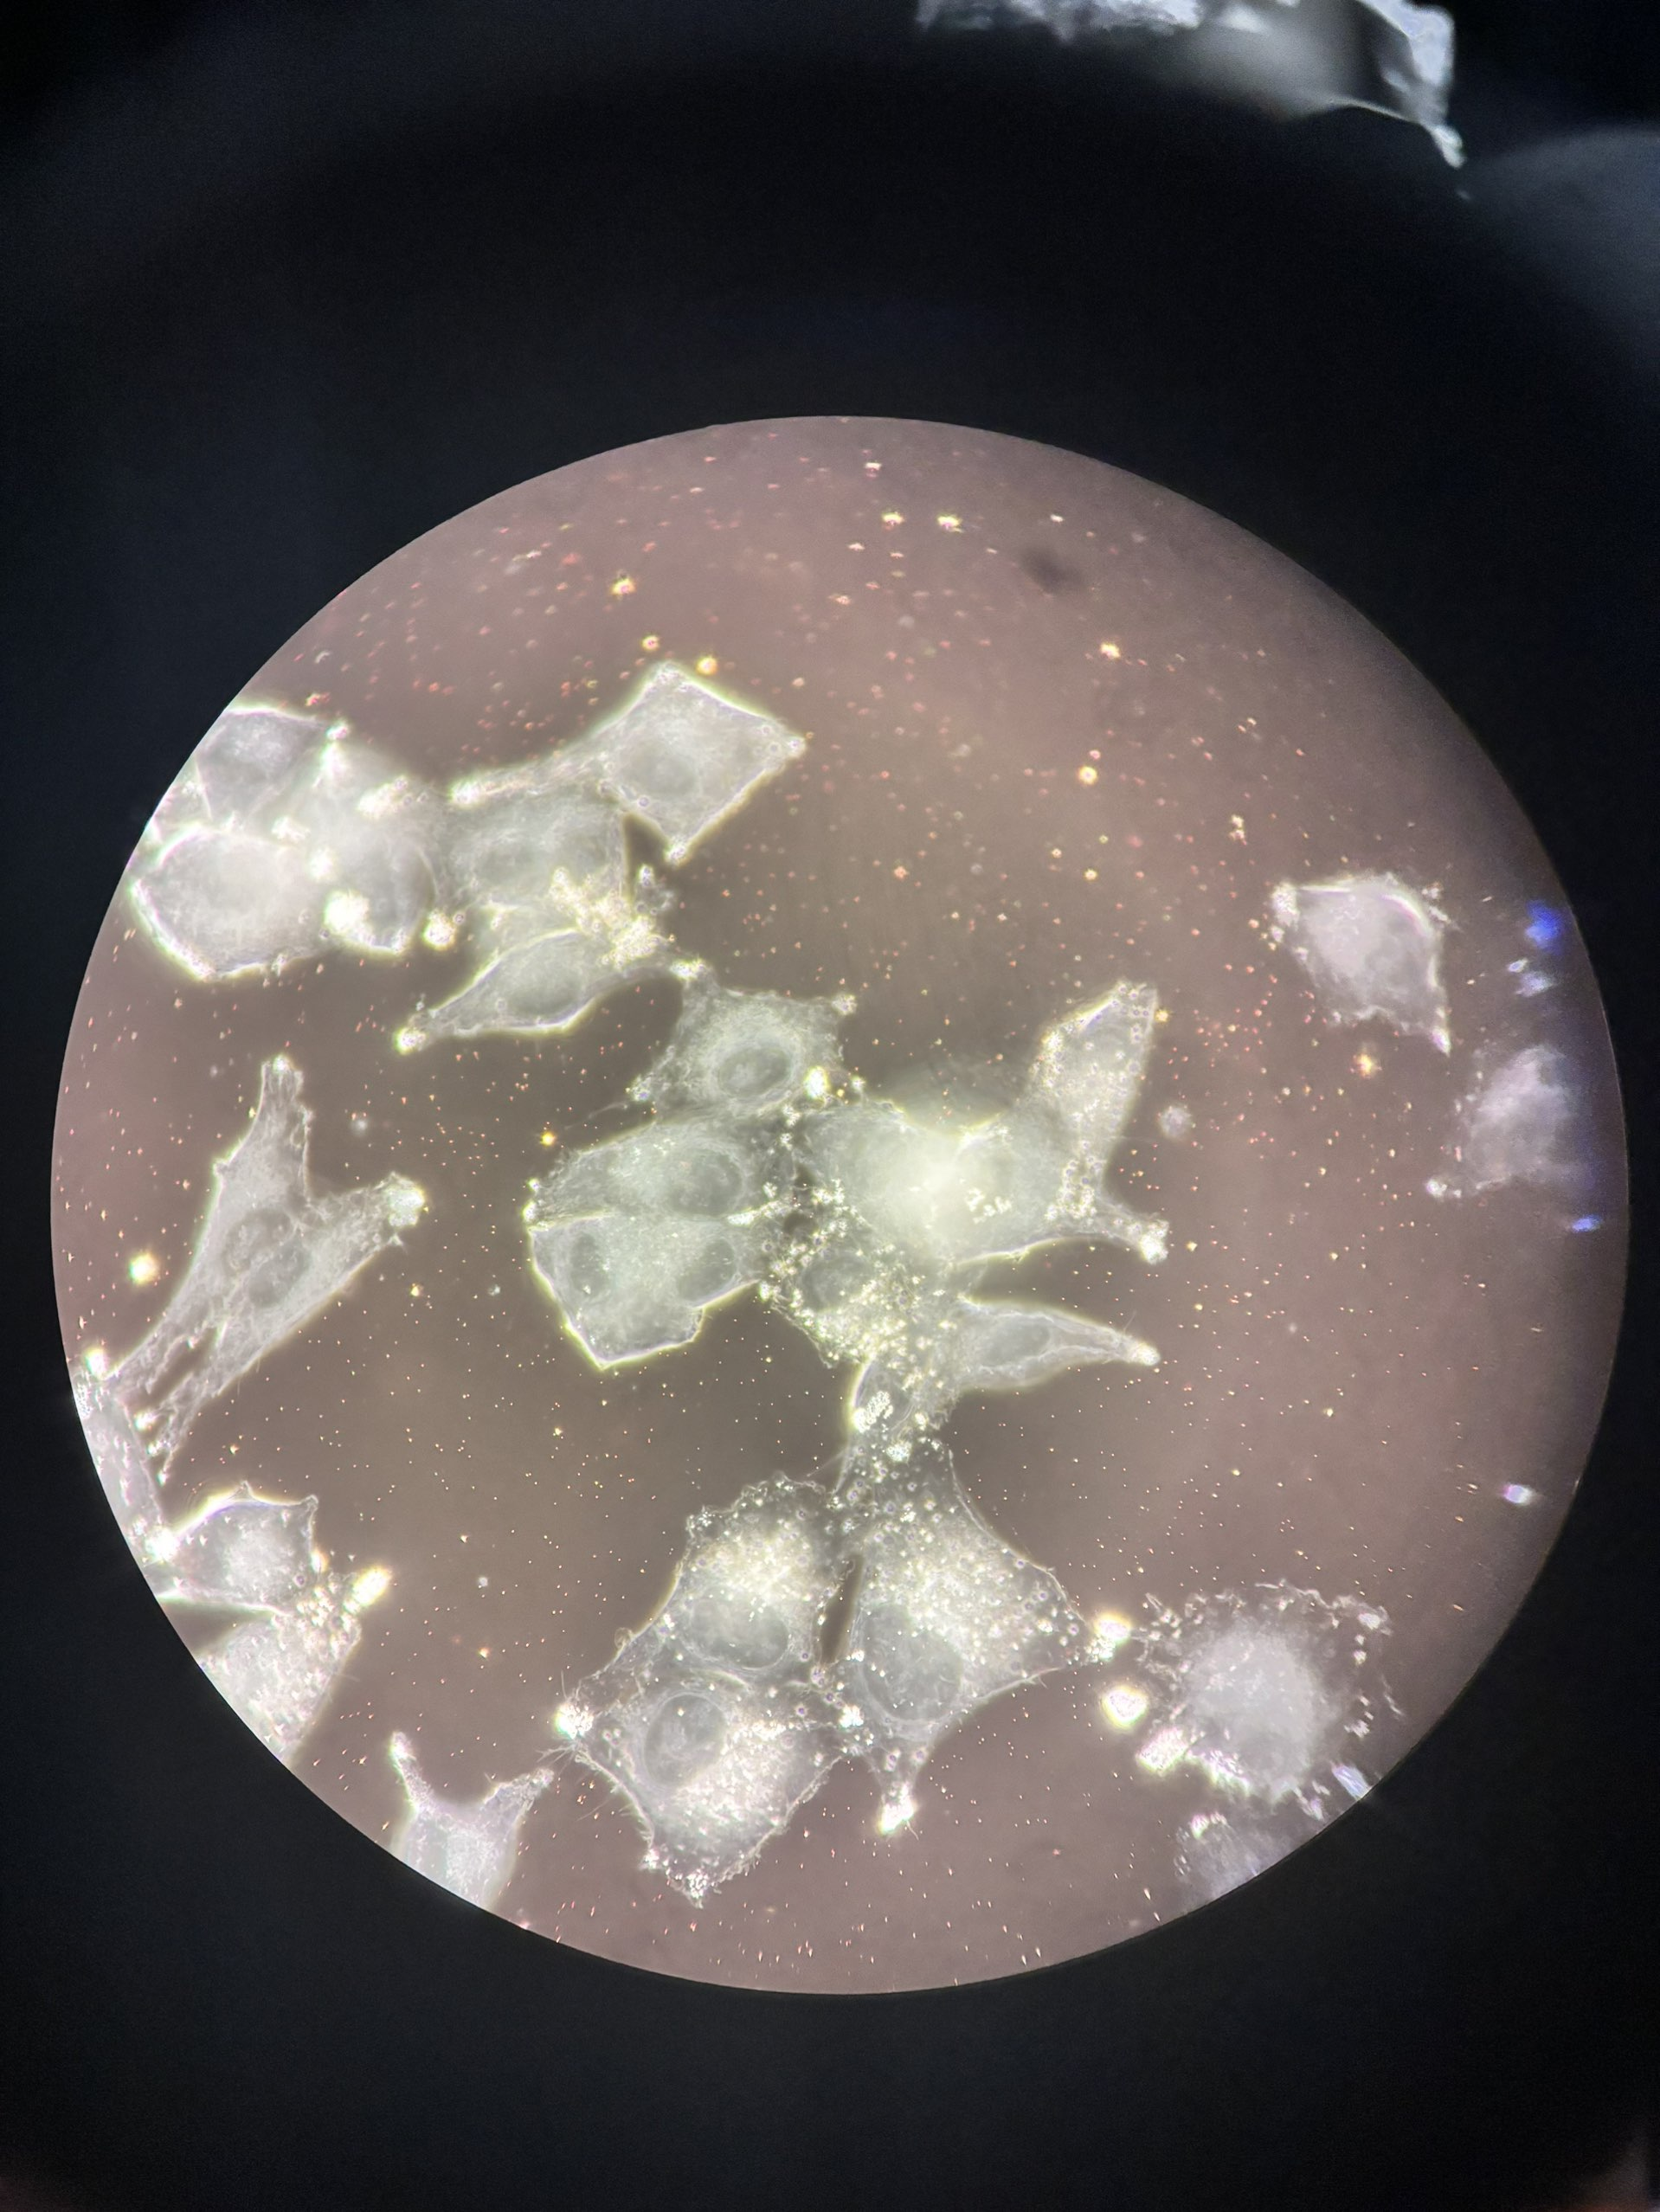
\includegraphics[width=\linewidth]{src/img/cell_darkfield_1.jpg}
  \end{minipage}\hfill
  \begin{minipage}{0.47\linewidth}
    \centering
    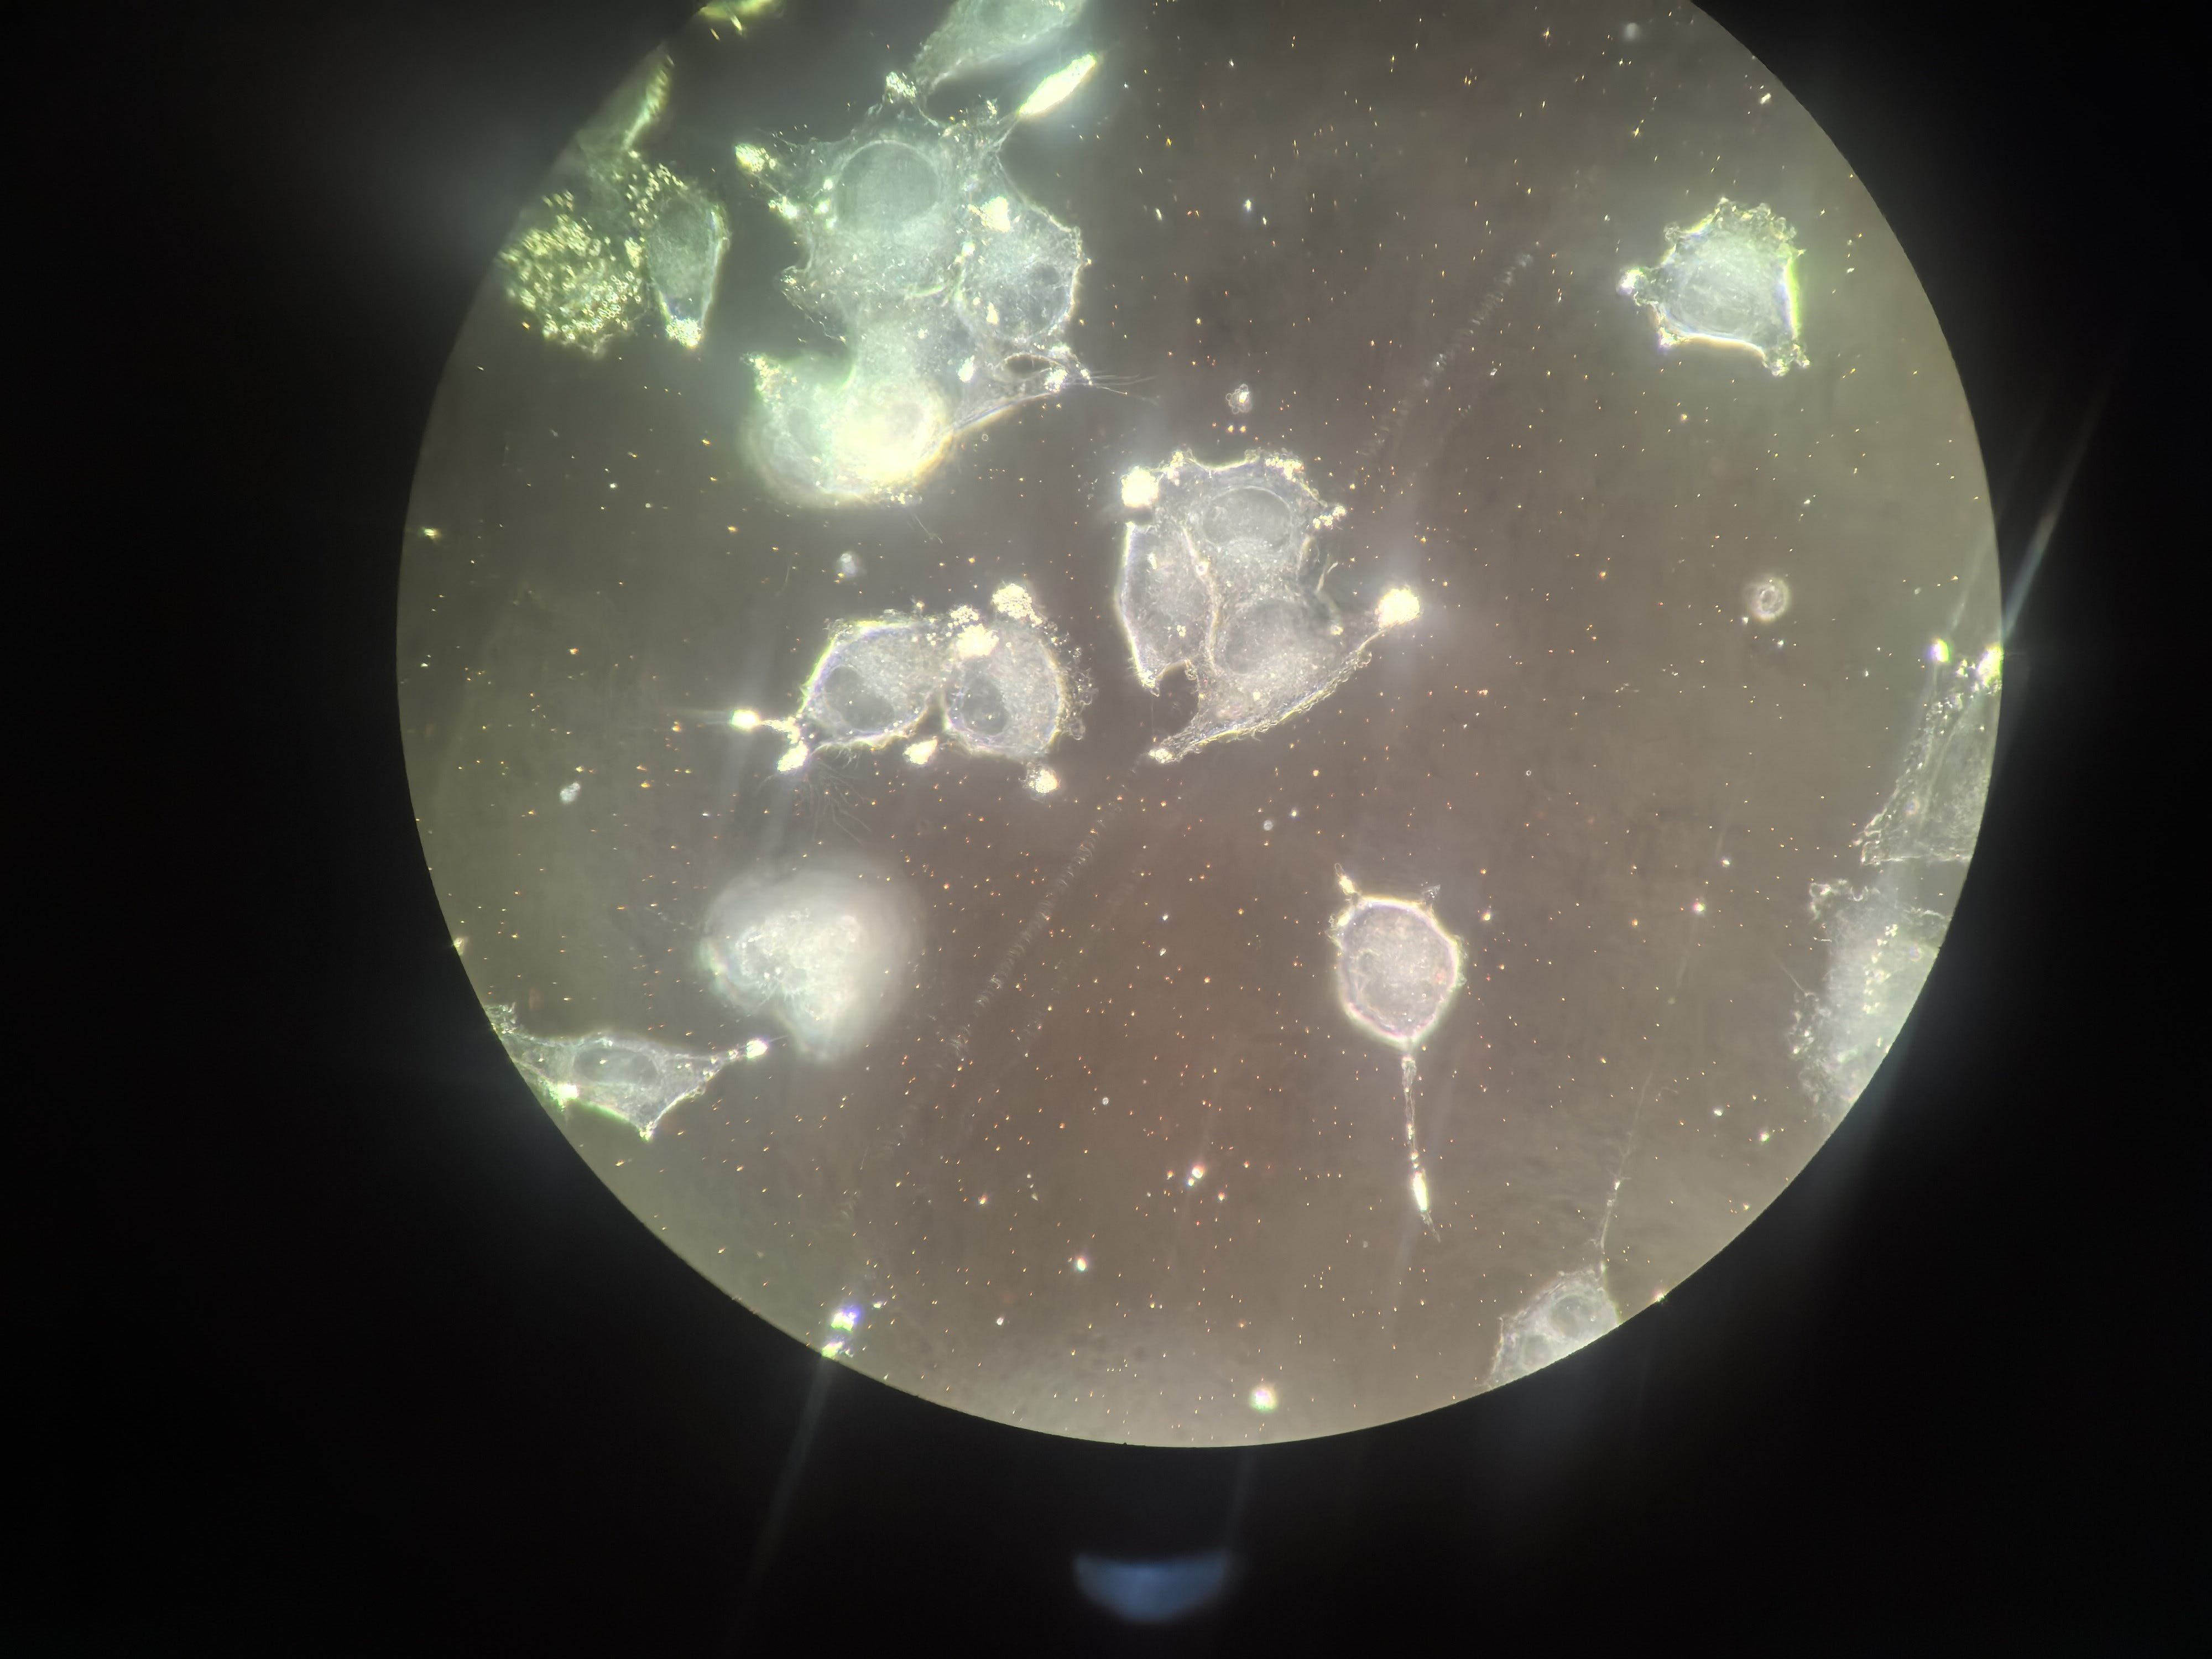
\includegraphics[width=\linewidth]{src/img/cell_darkfield_2.jpg}
  \end{minipage}
  \caption{{\zihaoWu 细胞样品的暗场显微成像。明亮区域对应细胞轮廓、细胞内散射结构及部分纳米颗粒信号。}}
  \label{fig:cell}
\end{figure}

从成像特点看，细胞膜表面颗粒密度通常高于远离细胞的背景区域，这是颗粒吸附、受体结合或内吞前富集的结果；随着孵育和内吞过程进行，胞内亮点比例增加，而培养基中游离颗粒相对减少。由于暗场图像只能给出散射强度和二维投影位置，若需进一步定量区分膜外、膜表面和胞内颗粒，仍需结合焦面扫描、荧光共定位或三维追踪方法。

\subsection{纳米颗粒运动轨迹的 MSD 展示}

考虑到第 3 组和第 4 组原始 MSD 曲线波动较大、呈现明显平台或周期性扰动，本报告不展示这两组数据。图\ref{fig:matlab_msd}保留第 1 组、第 2 组、第 3-2 组和第 4-2 组 MATLAB 直接输出的 MSD 拟合图，用于比较不同轨迹的基本形态。可以看出，第 1 组和第 4-2 组位移幅度较大，第 2 组后期趋于平台，第 3-2 组曲线随时间较稳定上升，拟合表现相对更适合用于后续详细分析。

\begin{figure}[htbp]
  \centering
  \begin{minipage}{0.48\linewidth}
    \centering
    
\includegraphics[width=\linewidth]{src/img/Figure_1.png}
    \centerline{{\zihaoXiaoWu (a) 第 1 组}}
  \end{minipage}\hfill
  \begin{minipage}{0.48\linewidth}
    \centering
    
\includegraphics[width=\linewidth]{src/img/Figure_2.png}
    \centerline{{\zihaoXiaoWu (b) 第 2 组}}
  \end{minipage}

  \vspace{0.5em}
  \begin{minipage}{0.48\linewidth}
    \centering
    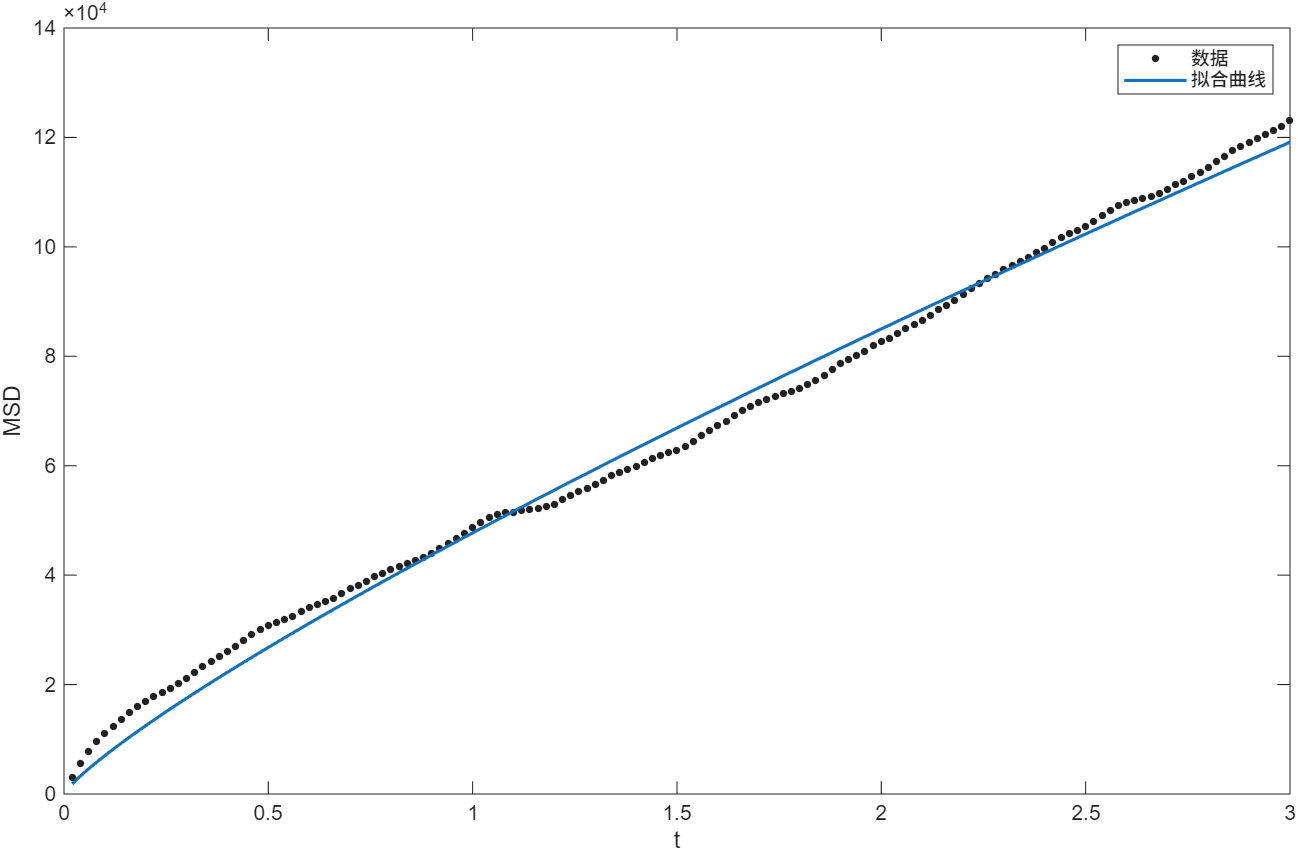
\includegraphics[width=\linewidth]{src/img/Figure_3-2.png}
    \centerline{{\zihaoXiaoWu (c) 第 3-2 组}}
  \end{minipage}\hfill
  \begin{minipage}{0.48\linewidth}
    \centering
    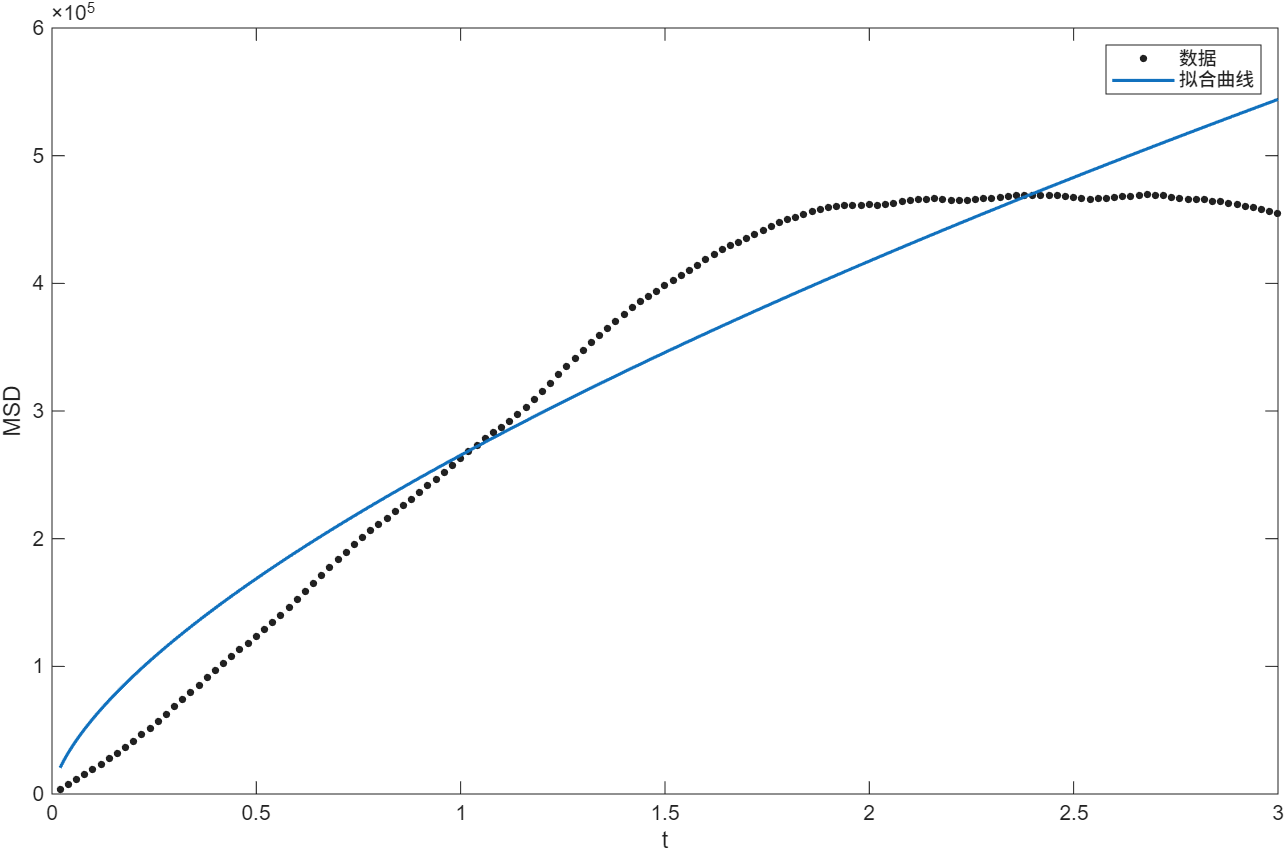
\includegraphics[width=\linewidth]{src/img/Figure_4-2.png}
    \centerline{{\zihaoXiaoWu (d) 第 4-2 组}}
  \end{minipage}
  \caption{{\zihaoWu MATLAB 直接输出的代表性颗粒 MSD--时间曲线及幂律拟合结果。}}
  \label{fig:matlab_msd}
\end{figure}

\begin{table}[htbp]
  \centering
  \caption{{\zihaoXiaoWu 代表性轨迹的表观扩散参数和异常扩散指数}}
  \label{tab:selected_diffusion}
  {\zihaoLiu
    \begin{tabular}{ccccc}
      \toprule
      轨迹      & 轨迹帧数 & 拟合时间/s & $D$/(nm$^2$ s$^{-\alpha}$) & $\alpha$ \\
      \midrule
      第 1 组   & 582  & 3.00   & $1.36\times10^{5}$         & 0.479    \\
      第 2 组   & 1000 & 3.00   & $8.65\times10^{3}$         & 0.309    \\
      第 3-2 组 & 1000 & 3.00   & $1.19\times10^{4}$         & 0.833    \\
      第 4-2 组 & 379  & 3.00   & $6.63\times10^{4}$         & 0.654    \\
      \bottomrule
    \end{tabular}}
\end{table}

\begin{figure}[htbp]
  \centering
  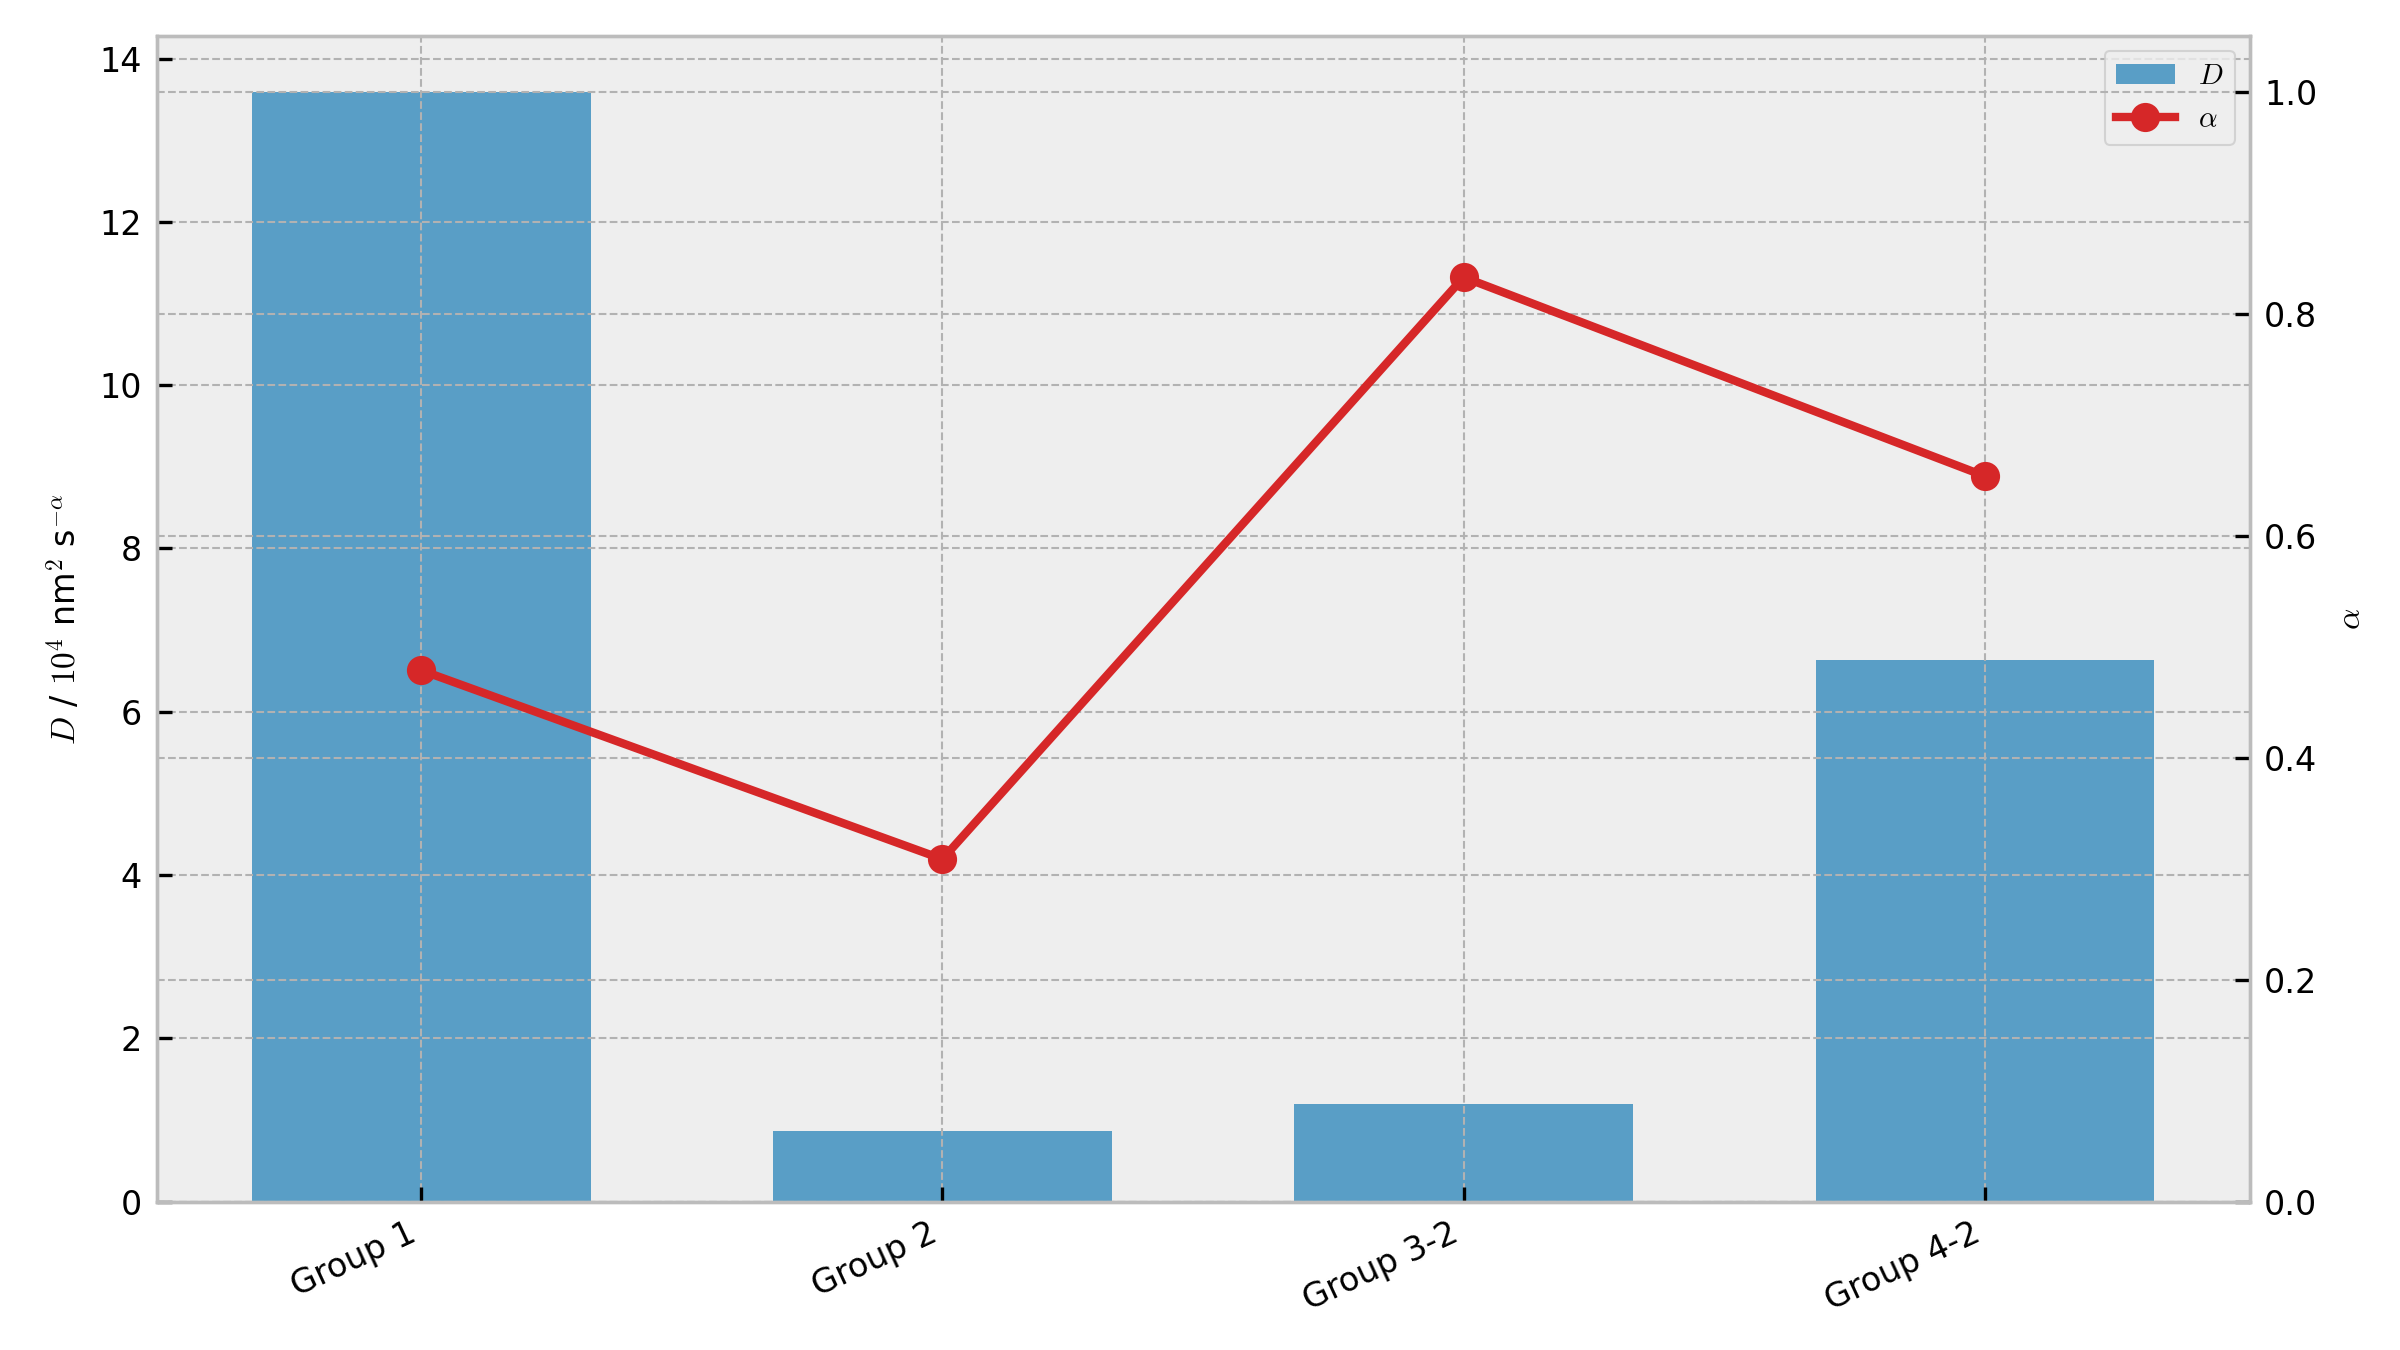
\includegraphics[width=0.74\linewidth]{src/img/diffusion_alpha_bmh.png}
  \caption{{\zihaoWu 代表性轨迹表观扩散参数 $D$ 与异常扩散指数 $\alpha$ 的比较。}}
  \label{fig:bar}
\end{figure}

表\ref{tab:selected_diffusion}和图\ref{fig:bar}显示，不同轨迹之间的表观扩散参数差异较大，说明暗场追踪得到的运动行为不仅与颗粒本身尺寸、形貌有关，也与颗粒所处的细胞膜区域、焦面稳定性和局部背景有关。第 1 组 $D$ 最大但 $\alpha$ 低于 0.5，说明短时间位移幅度较大但受限特征明显；第 2 组 $\alpha$ 更低，提示后期可能出现局域束缚或追踪范围受限；第 4-2 组 $D$ 和 $\alpha$ 均较高，但轨迹较短，结果受轨迹长度影响更大。因此，后文重点讨论曲线形态较平滑、轨迹长度较充分且 $\alpha$ 接近弱受限扩散区间的第 3-2 组。

\subsection{第 3-2 组轨迹的详细讨论}

第 3-2 组轨迹共记录 1000 帧，按 0.02~s 的帧间隔计算，以前 150 个时间间隔进行拟合，对应拟合时间范围为 0--3.00~s。该组数据的 MSD 随时间基本单调增加，且散点与拟合曲线整体符合较好，说明该轨迹在所选时间窗口内具有较稳定的扩散趋势，适合作为细胞膜表面颗粒运动的代表性分析对象。

由表\ref{tab:selected_diffusion}可知，第 3-2 组拟合得到的表观扩散参数 $D=1.19\times10^{4}$~nm$^2$~s$^{-\alpha}$，异常扩散指数 $\alpha=0.833$。若以 $MSD(t)=4Dt^{\alpha}$ 估算，在 $t=3.00$~s 时 MSD 约为 $1.2\times10^{5}$~nm$^2$，对应均方根位移约 $3.5\times10^{2}$~nm。该位移量级显著大于单个纳米颗粒尺寸，说明颗粒并非完全固定在某一点；但 $\alpha$ 明显小于 1，又说明其运动并非理想自由布朗扩散，而是具有亚扩散特征。

从物理意义上看，$\alpha$ 介于 0.5 与 1 之间通常可理解为弱受限异常扩散。对于细胞膜表面的纳米颗粒，这种行为可能来自多个因素：其一，颗粒与膜表面蛋白、糖链或局部受体之间存在短暂结合，使颗粒运动呈现“移动--停留--再移动”的间歇特征；其二，细胞膜骨架和脂筏等微区会形成空间障碍，使颗粒在一定区域内被限制但未完全固定；其三，颗粒可能处于膜外近表面、膜表面吸附和内吞早期之间的过渡状态，因此轨迹既具有随机扩散成分，也受到细胞主动过程和局部黏滞环境影响。

第 3-2 组 MSD 曲线在短时间段内上升较快，随后仍保持近似线性增长，没有明显进入平台区。这说明在 3~s 的观测窗口内，颗粒尚未被严格限制在封闭小区域内，其可探索空间仍随时间扩大。与此同时，拟合曲线相对于理想线性布朗扩散呈次线性增长，表明扩散能力随观测时间延长有所减弱。若继续延长追踪时间，可能会观察到更明显的平台、方向性转运或内吞后沿细胞骨架运动等特征。

该分析也存在一定局限。暗场散射光斑尺寸大于颗粒真实尺寸，中心定位容易受背景细胞结构、焦面漂移和信噪比影响；二维轨迹忽略了 $z$ 轴方向的离焦运动，因而只能得到投影平面内的表观扩散参数；此外，幂律模型将复杂的膜表面运动平均化为两个参数，不能单独区分受体结合、膜微区限制和细胞主动运输等机制。尽管如此，第 3-2 组较平滑的 MSD 增长和较高的 $\alpha$ 值仍表明，该颗粒更接近弱受限扩散状态，是讨论纳米颗粒在细胞膜表面运动行为的较合适样本。

\section{思考题}
\vspace{-0.5em}

\subsection{取几幅采集的纳米颗粒暗场成像图，通过颜色、大小等信息鉴别出四种纳米颗粒。}

四种纳米颗粒可依据暗场图像中的形貌和散射颜色综合判断。球形金纳米颗粒主要呈点状明亮散射，55~nm 金纳米颗粒对应绿色点状信号，60~nm 金纳米颗粒对应蓝色点状信号；25$\times$60~nm 金纳米棒因长径比较小，表现为黄色短棒状散射；40$\times$80~nm 金纳米棒长径比较大，纵向 LSPR 进一步红移，表现为更明显的橙红色长棒状散射。实际判别时不能只依赖单个颗粒的颜色，还应结合多个颗粒的平均形貌、亮度和运动状态，避免将聚集颗粒或离焦光斑误认为棒状颗粒。

\subsection{通过对比紫外可见吸收光谱、电镜表征和暗场成像，并查阅相关资料，讨论三者技术的优缺点。}

紫外--可见吸收光谱操作快速、无损且适合批量检测，可通过 LSPR 吸收峰位置和峰形初步判断纳米颗粒的尺寸、形貌和聚集程度，但它给出的是群体平均信息，无法观察单颗粒差异，也不能直接提供空间分布。电镜表征分辨率最高，能够直接测量颗粒尺寸、形貌、长径比和分散性，是结构确认的可靠手段；但其制样复杂、测试成本高，通常需要干燥或真空环境，难以反映液相和活细胞中的原位动态过程。暗场成像分辨率低于电镜，但可在液相、活细胞和较接近真实应用环境下观察单颗粒散射信号，尤其适合研究颗粒运动、扩散和细胞相互作用；其不足是散射颜色受焦面、背景、颗粒聚集和光学系统影响较大，定量尺寸判断不如电镜精确。

\subsection{探讨金、银纳米颗粒在细胞膜内、外及表面的粒子密度。}

在加入纳米颗粒后的初始阶段，膜外培养基中游离颗粒密度较高，颗粒在溶液中以随机布朗运动为主。随着孵育进行，部分颗粒通过静电作用、配体--受体作用或非特异性吸附富集到细胞膜表面，因此膜表面局部颗粒密度升高，暗场图像中可观察到细胞边缘和膜附近亮点增多。进一步孵育后，一部分颗粒可能经内吞进入细胞内部，胞内颗粒密度逐渐增加。通常小尺寸球形颗粒更容易接近膜表面并被内吞，较大颗粒或长棒状颗粒受空间位阻和取向影响，内吞效率可能较低。由于金纳米颗粒散射信号较稳定，暗场下更易被识别；银纳米颗粒亮度和稳定性受尺寸、氧化或聚集影响更明显，密度估算时应校正成像灵敏度差异。

\subsection{探讨金、银纳米颗粒在细胞膜表面扩散运动的情况（扩散轨迹、速率等）。}

纳米颗粒在细胞膜表面的扩散轨迹通常不是理想的无限自由布朗运动。未与膜强结合的颗粒可呈现较大范围的随机游走，MSD 随时间接近线性增加；与膜蛋白、受体或糖链发生相互作用后，轨迹会表现为局域徘徊、短暂停顿或在有限区域内扩散，MSD 增长变慢并出现亚扩散特征；若颗粒进入内吞或被细胞骨架相关结构牵引，还可能出现方向性位移。扩散速率受颗粒尺寸、形貌、表面电荷、材料组成以及细胞膜状态影响。一般来说，小颗粒受到的流体阻力和空间位阻较小，表观扩散较快；长棒状颗粒转动和取向限制更强，扩散可能较慢；膜流动性下降、受体结合增强或细胞骨架限制增强时，扩散系数会降低，异常扩散指数也会小于 1。通过单颗粒追踪计算 MSD 并拟合 $MSD(t)=4Dt^{\alpha}$，可对这种扩散状态进行定量表征。

\section{结论}
\vspace{-0.5em}

本实验利用暗场显微成像观察了不同形貌金属纳米颗粒和细胞样品。结果表明，暗场图像中的散射颜色和形状可有效区分球形纳米颗粒与金纳米棒；长径比增加会导致金纳米棒纵向 LSPR 红移，使散射颜色向橙红色变化。细胞暗场成像显示纳米颗粒可富集于细胞膜相关区域，并呈现不同程度的受限运动。

代表性轨迹比较显示，第 1 组、第 2 组、第 3-2 组和第 4-2 组的 MSD 行为存在明显差异，其中第 3-2 组曲线增长较稳定，更适合展开定量讨论。对第 3-2 组单颗粒轨迹的 MSD 分析表明，该颗粒的 $D$ 为 $1.19\times10^{4}$~nm$^2$~s$^{-\alpha}$，$\alpha$ 为 0.833，属于弱受限异常扩散。该结果说明颗粒在细胞膜相关区域仍具有明显移动能力，但其运动受到膜结构、局部结合和细胞微环境的限制，不同于自由溶液中的理想布朗扩散。后续可结合三维单颗粒追踪、荧光共定位或不同表面修饰颗粒的对比实验，进一步阐明纳米颗粒跨膜吸附、扩散和内吞机制。

\vspace{3em}
{\footnotesize
  \setstretch{1}
  \begin{thebibliography}{9}
    \bibitem{eustis2006}
    Eustis S, El-Sayed M A. Why gold nanoparticles are more precious than pretty gold: Noble metal surface plasmon resonance and its enhancement of the radiative and nonradiative properties of nanocrystals of different shapes. \textit{Chem. Soc. Rev.}, \textbf{2006}, 35: 209--217.

    \bibitem{murphy2005}
    Murphy C J, Sau T K, Gole A M, et al. Anisotropic metal nanoparticles: Synthesis, assembly, and optical applications. \textit{J. Phys. Chem. B}, \textbf{2005}, 109: 13857--13870.

    \bibitem{kusumi1993}
    Kusumi A, Sako Y, Yamamoto M. Confined lateral diffusion of membrane receptors as studied by single particle tracking. \textit{Biophys. J.}, \textbf{1993}, 65: 2021--2040.

    \bibitem{kowalek2019}
    Kowalek P, Loch-Olszewska H, Szwabiński J. Classification of diffusion modes in single-particle tracking data: Feature-based versus deep-learning approach. \textit{Phys. Rev. E}, \textbf{2019}, 100: 032410.

    \bibitem{paramelle2014}
    Paramelle D, Sadovoy A, Gorelik S, Free P, Hobley J, Fernig D G. A rapid method to estimate the concentration of citrate capped silver nanoparticles from UV-visible light spectra. \textit{Analyst}, \textbf{2014}, 139: 4855--4861.
  \end{thebibliography}
}

\vspace*{\fill}
\noindent{\zihaoWu 评语（Remarks）：}

\vspace{2em}

\begin{center}
  {\zihaoWu\bfseries 指导教师（Instructor）\hspace{8em} 日期（Date）}
\end{center}

\vspace{1.5cm}

\end{document}
